\documentclass{standalone}

\usepackage{tikz}
\usepackage{bm}

\usetikzlibrary{decorations.markings}

\begin{document}

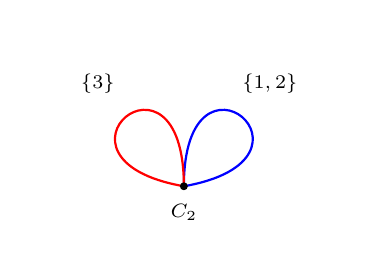
\begin{tikzpicture}

\begin{scope}[xscale=1, yscale=1, thick]

\def\loopangle{10}
\def\loopsize{2}
\def\looplabelsep{0}
\def\vertexlabelsep{1mm}

\def\nrloops{2}
\draw [blue] (0:0) .. controls ({\loopangle+0*(180-2*\loopangle)/\nrloops}:\loopsize) and ({\loopangle+1*(180-2*\loopangle)/\nrloops}:\loopsize) .. (0:0);
\node at ({\loopangle+0*(180-2*\loopangle)/\nrloops+(180-2*\loopangle)/\nrloops/2}:\loopsize-0.3+\looplabelsep) {\scriptsize{$\{ 1, 2 \}$}};

\draw [red] (0:0) .. controls ({\loopangle+1*(180-2*\loopangle)/\nrloops}:\loopsize) and ({\loopangle+2*(180-2*\loopangle)/\nrloops}:\loopsize) .. (0:0);
\node at ({\loopangle+1*(180-2*\loopangle)/\nrloops+(180-2*\loopangle)/\nrloops/2}:\loopsize-0.3+\looplabelsep) {\scriptsize{$\{ 3 \}$}};

\node (0) at (0:0) {};
\draw [fill] (0) circle [radius=1pt];
\node [below=\vertexlabelsep] at (0) {\scriptsize{$C_{2}$}};

\end{scope}

\end{tikzpicture}

\end{document}

